\documentclass[12pt]{article}
\usepackage[left=3cm, top=1cm, right=3cm, bottom=3cm]{geometry}
\usepackage[utf8]{inputenc}      % accents dans le source
\usepackage[T1]{fontenc}
\usepackage[french]{babel}
\usepackage{graphicx}
\usepackage{graphics}
\usepackage{amsmath}
\usepackage{tikz}
\usepackage{xcolor} 
\usepackage{mathtools}
\usepackage{parskip}
\usepackage{subcaption}
\usepackage[export]{adjustbox}
\usepackage{chemist}
\usepackage{rotating}
\usepackage{hyperref}
\hypersetup{colorlinks=true,linkcolor=blue}

\title{\textbf{TP Cinétique} \\Étude cinétique de la réaction entre le bleu de bromophénol et l'ion hydroxyde}
\author{MENARD Alexandre \\ VIEILLEDENT Florent}

\begin{document}
\maketitle

\section*{Introduction}
Dans ce travail pratique on étudie la cinétique de la réaction entre le bleu de bromophénol et l'hydroxyde.
On suit l'avancement de la réaction par spectrophotomètrie.

\section{Température ambiante}

\textbf{Question 1 :} On calcule la concentration initiale de la solution en BBP. 
La solution utilisée est à $0.4 \ g.L^{-1}$ ce qui correspond à $C_0=5.97\times 10^{-4} \ mol.L^{-1}$, la masse molaire du BBP étant de $669.5 \ g.mol^{-1}$.
On dilue 2 mL de cette solution dans une solution d'hydroxyde qu'on étent à 50mL, on a donc $C=\frac{C_0 \times V_0}{V}=\frac{5.97\times 10^{-4}\times 2}{50}=2.39\times 10^{-5}\ mol.L^{-1}$.

\textbf{Question 2 :} On a pour l'incertitude :
\begin{align*}
    \Delta C &= C \times \left( \frac{\Delta C_0}{C_0} + \frac{\Delta V_0}{V_0} + \frac{\Delta V}{V} \right) \\
    \Delta C &= 2.93\times 10^{-5} \times \left( 0.005 + 0.004 + 0.001 \right) \\
    \Delta C &= 3\times 10^{-7} \ mol.L^{-1}
\end{align*}

\textbf{Question 3 :} On a finalement $C= 2.93 \pm 0.03 \times 10^{-5}\ mol.L^{-1}$.

\textbf{Question 4 :} La solution utilisée pour régler le zéro d'absorbance est la solution d'hydroxyde à $1.4 \ mol.L^{--1}$.

\textbf{Question 5 :} On mesure la température de la pièce à $T_1 = 22 \pm 2 ^\circ C$. 
L'incertitude sur la température est donnée par la thermomètre et le fait qu'on ne contrôle pas la température de la pièce pendant l'expérience.

\textbf{Question 6 :} On mesure pour notre premier une absorbance $A_0=1.15\pm 0.02$. L'incertitude est donnée par le spectrophotomètre et en prenant en compte que l'absorbance varie rapidement au début de l'expérience.
Cette valeur est obtenue pour un temps de 45 secondes, la concentration de BBP a eu le temps de diminuer significativement notre valeur de $\epsilon_{\lambda Bmax}$ ne sera donc pas très précise.
Pour obtenir une valeur plus précise il faut extrapoler nos données jusqu'à $t=0$.
D'après la loi de Beer-Lambert, en utilisant une cuve de 1 cm :
\begin{align*}
    \epsilon_{\lambda Bmax} &= \frac{A_0}{C} \\
    \epsilon_{\lambda Bmax} &= \frac{1.15}{2.93\times 10^{-5}} \\
    \epsilon_{\lambda Bmax} &= 3.93 \times 10^4 \ L.mol^{-1}.cm^{-1}
\end{align*}

\textbf{Question 7 :} On calcule l'incertitude :
\begin{align*}
    \Delta  \epsilon_{\lambda Bmax} &=  \epsilon_{\lambda Bmax} \times \left(\frac{\Delta C}{C} + \frac{\Delta A}{A} \right) \\
    \Delta  \epsilon_{\lambda Bmax} &=  3.93 \times 10^4 \times \left( \frac{0.03}{2.93} \frac{0.02}{1.15}  \right) \\
    \Delta  \epsilon_{\lambda Bmax} &= 0.1 \times 10^4 \ L.mol^{-1}.cm^{-1}
\end{align*}

\textbf{Question 8 :} On a $\epsilon_{\lambda Bmax} =4.0 \pm 0.1 \times 10^4 \ L.mol^{-1}.cm^{-1}$.

\textbf{Question 9 :} Pour trouver la concentration en tout instant on utlise la relation : $[BBP](t)=\frac{A(t)}{\epsilon_{\lambda Bmax}}=\frac{A(t)\times C}{A_0}$.
On prend une incertitude sur le temps de 2 secondes.
\begin{table}[h!]
\begin{center}
    \begin{tabular}{|c|c|c|}
        \hline
        $Absorbance \pm 0.02 $ & Concentration en mol/L & Temps $\pm$ 0.033 en min \\
        \hline
                    1.15 &             0.00002400 &             0.75 \\
                    1.09 &             0.00002271 &             1.066 \\
                    1.05 &             0.00002198 &             2.266 \\
                    1.02 &             0.00002125 &             2.750 \\
                    0.96 &             0.00002010 &             3.466 \\
                    0.91 &             0.00001915 &             4.083 \\
                    0.85 &             0.00001788 &             4.833 \\
                    0.81 &             0.00001698 &             5.466 \\
                    0.76 &             0.00001594 &             6.283 \\
                    0.75 &             0.00001565 &             7.166 \\
                    0.66 &             0.00001394 &             9.000 \\
                    0.62 &             0.00001298 &            10.016 \\
                    0.58 &             0.00001210 &            10.916 \\
                    0.54 &             0.00001144 &            11.966 \\
                    0.50 &             0.00001060 &            12.883 \\
                    0.43 &             0.00000915 &            13.783 \\
                    0.39 &             0.00000821 &            15.333 \\
                    0.36 &             0.00000754 &            16.700 \\
                    0.33 &             0.00000688 &            17.933 \\
                    0.30 &             0.00000644 &            20.983 \\
                    0.28 &             0.00000598 &            21.916 \\
                    0.27 &             0.00000569 &            23.166 \\
                    0.25 &             0.00000525 &            25.266 \\
        \hline
        \end{tabular}
        \caption{Tableau des valeurs de la concentration et de l'absorbance pour les différents temps}
        \label{table1}
\end{center}
\end{table}
\newpage
\textbf{Question 10:}
On trace [BBP], $ln \left(\frac{[BBP]}{[BBP]_0}\right)$ et $\frac{1}{[BBP]}$ en fonction du temps.

\begin{figure}[h!]
    \begin{center}
        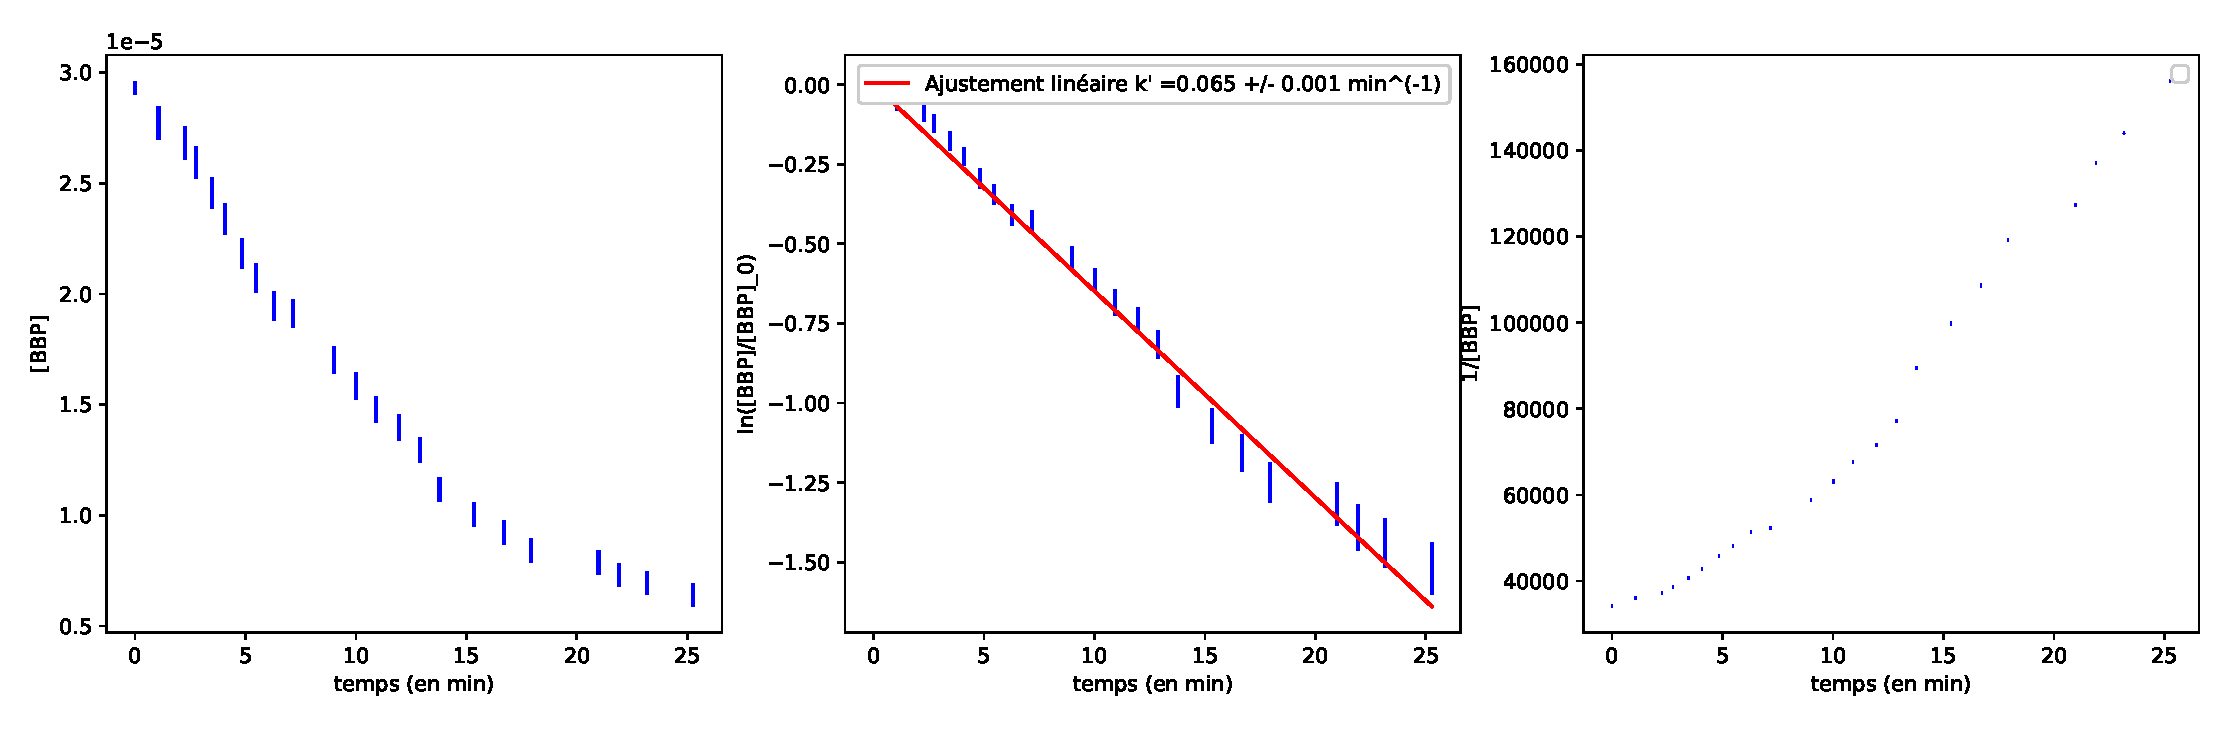
\includegraphics[width=1\linewidth]{3CourbesCinétiques.eps}
        \caption{Courbes de gauche à droite : [BBP], $ln \left(\frac{[BBP]}{[BBP]_0}\right)$ et $\frac{1}{[BBP]}$ en fonction du temps. On a rajouté l'ajustement linéaire pour la deuxième courbe}
        \label{img:3courbes}
    \end{center}
\end{figure}

On remarque qu'on obtient une droite lorsqu'on trace le logarithme sur le graphique (\ref{img:3courbes}).
On a donc l'ordre partiel $\alpha =1$ et on trouve $k'=0.065 \pm 0.001 min^{61}$.
\newpage
\textbf{Question 11 et 12 :} On trace $ln(k')$ en fonction de $ln([OH-])$ sur le graphique (\ref{img:lnk}). 
\begin{figure}[h!]
    \begin{center}
        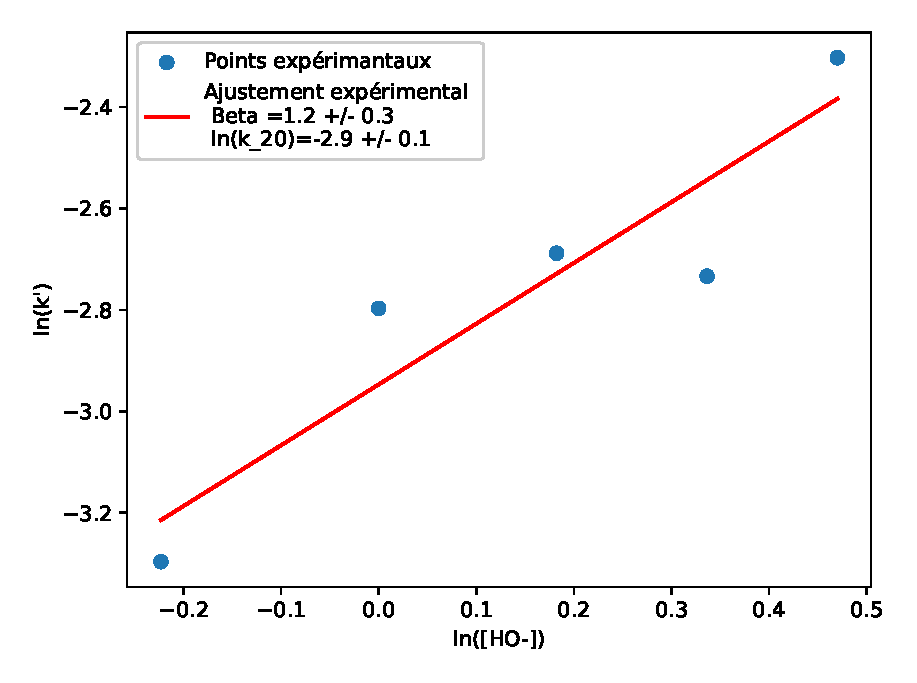
\includegraphics[scale=0.8]{Ln(k).eps}
        \caption{Graphique de $ln(k')$ en fonction de $ln([OH-])$ avec ajustement linéaire}
        \label{img:lnk}
    \end{center}
\end{figure}

On obtient une valeur de $k_{20 ^\circ C}=0.055 \pm 0.005 \ L.mol^{-1}.min^{-1}$.
On obtient une valeur de $\beta = 1.2 \pm 0.3$.
\newpage
\textbf{Question 13 :}
On calcule $t_{1/2}$ pour $[OH-]=1.4 mol.L^{-1}$. On obtient : $t_{1/2}=\frac{ln(2)}{k'}=\frac{ln(2)}{0.065}=11 min$.
On trouve un résultat cohérent sur le graphique:
\begin{figure}[h!]
    \begin{center}
        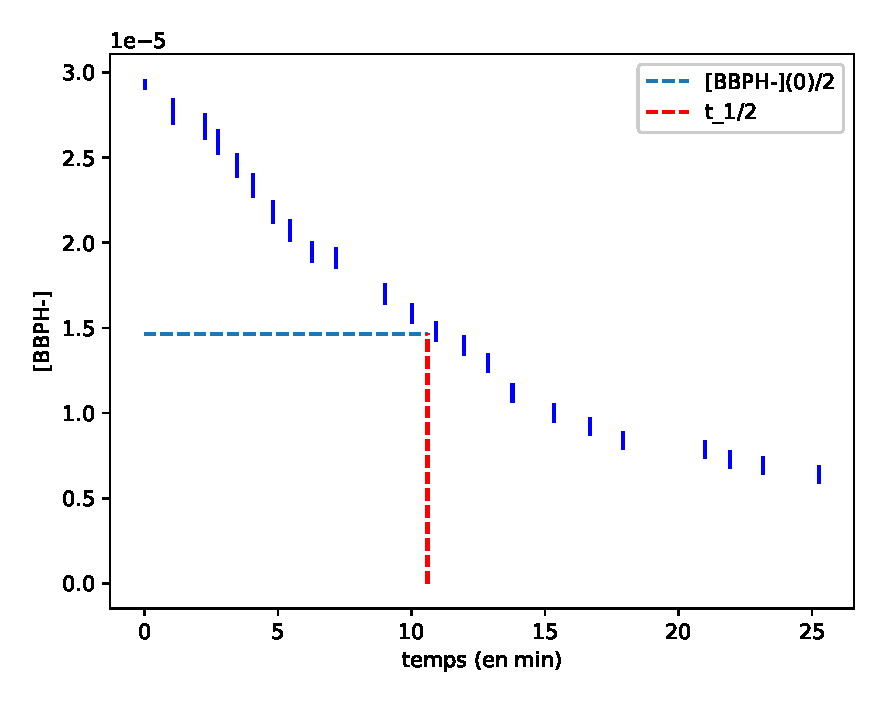
\includegraphics[scale=0.7]{demivie.eps}
        \caption{Vérifaction de la valeur calculée de $t_{1/2}$}
        \label{img3:demivie}
    \end{center}
\end{figure}

\textbf{Question 14 :} Nous avons calculé les ordres partiels égaux à 1 et $1.2\pm 0.3$ de la réaction et calculé les constantes de vitesse pour une température ambiante. 
On note que notre valeur de k' semble apperante sur le graphique(\ref{img:lnk}) par rapport aux autres points.
Cela peut venir d'une différence de température de la pièce et de notre méthode peu précise pour calculer $\epsilon_{\lambda Bmax}$. 

\newpage
\section{Glace fondante}
\textbf{Question 1 :} On répete les mêmes calcule que pour la première partie pour nos nouvelles données.
\begin{table}[h!]
    \begin{center}
        \begin{tabular}{|c|c|c|}
            \hline
        $Absorbance \pm 0.02 $ & Concentration en mol/L & Temps $\pm$ 0.033 en min \\
            \hline
                        1.46 &             0.00002490 &             0.75 \\
                        1.21 &             0.00002071 &             1.96 \\
                        1.36 &             0.00002330 &             2.88 \\
                        1.25 &             0.00002144 &             5.33 \\
                        1.17 &             0.00001994 &            10.08 \\
                        1.00 &             0.00001712 &            17.50 \\
                        1.07 &             0.00001833 &            21.58 \\
                        0.85 &             0.00001453 &            27.25 \\
                        0.82 &             0.00001407 &            30.75 \\
                        0.77 &             0.00001327 &            36.16 \\
                        0.69 &             0.00001179 &            41.25 \\
                        0.75 &             0.00001291 &            45.88 \\
                        0.63 &             0.00001080 &            49.58 \\
                        0.57 &             0.00000978 &            55.16 \\
                        0.56 &             0.00000954 &            58.16 \\
                        0.56 &             0.00000957 &            59.75 \\
            \hline
            \end{tabular}
    \end{center}
    \caption{Tableau de données pour la deuxième expérience}
\end{table}

\begin{figure}[h!]
    \begin{center}
        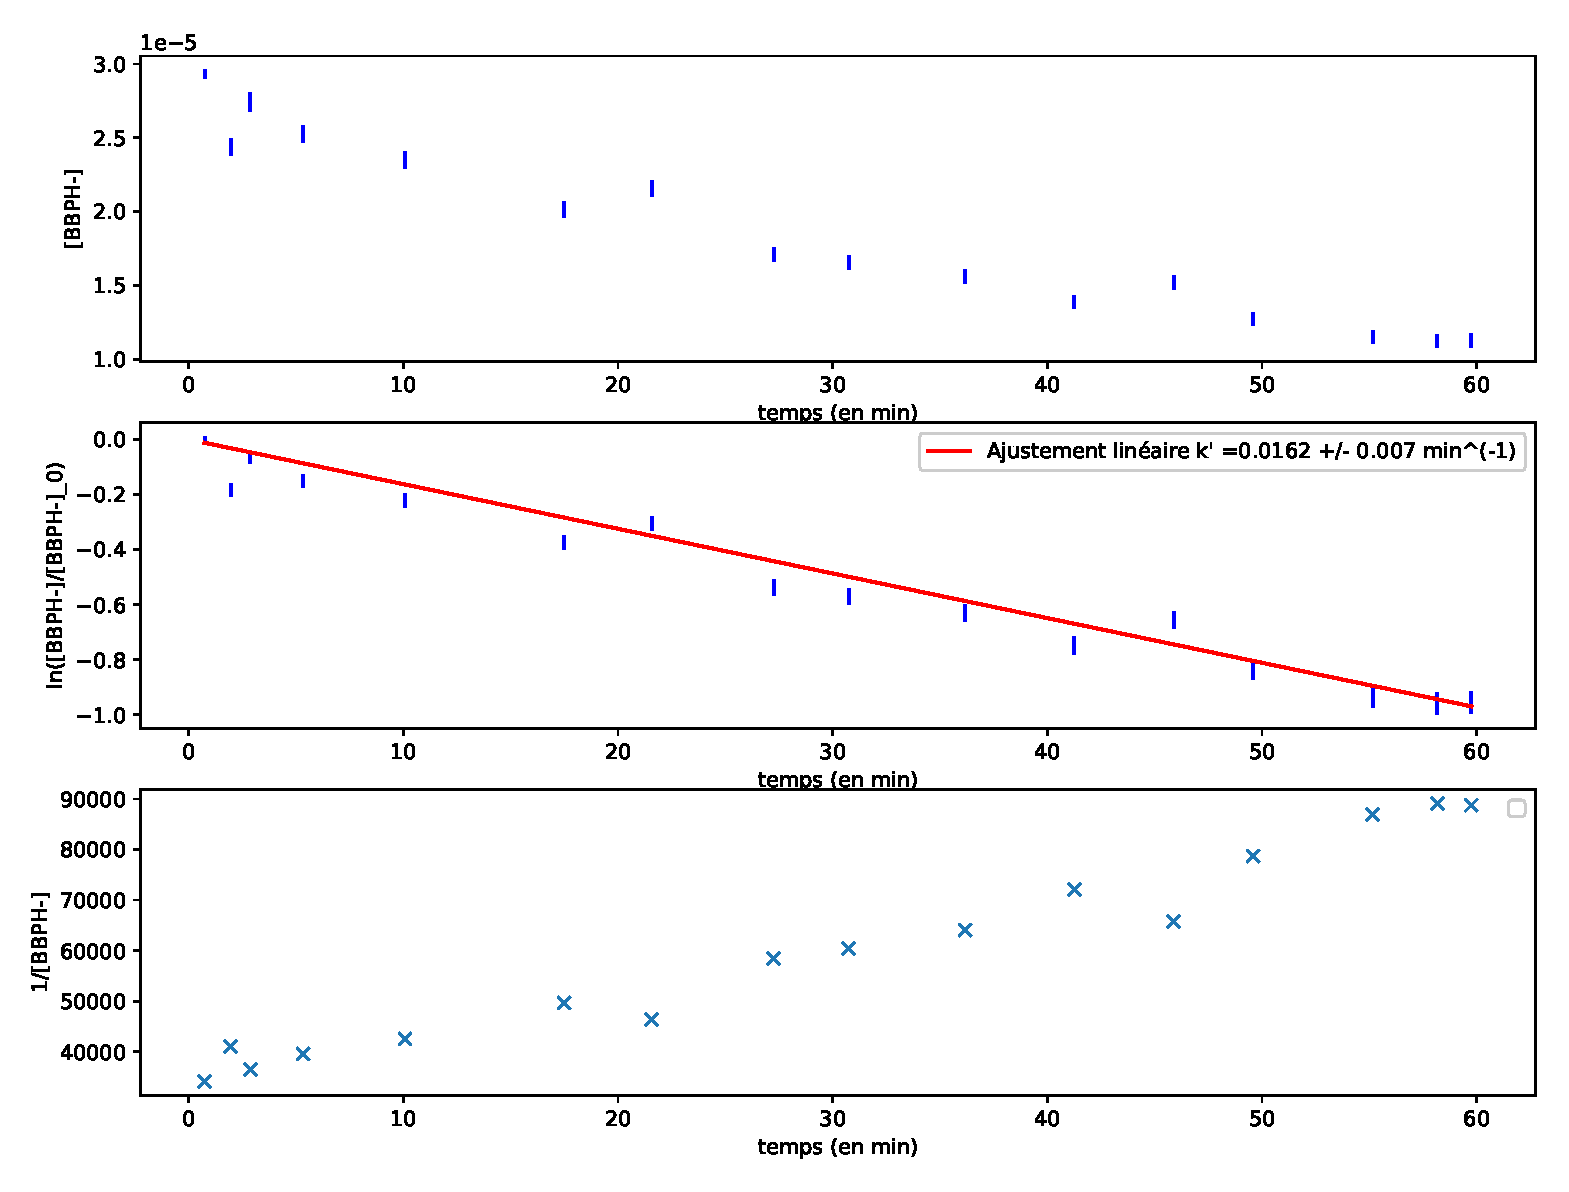
\includegraphics[scale=0.55]{DeuxièmeCourbesCinétiques.eps}
        \caption{Courbes de concentration pour la deuxième expérience}
        \label{img4:deuxièmexp}
    \end{center}
\end{figure}
Nos points ne sont pas très alignés même pour la courbe avec le logarithme. 
Cela peut venir d'un mauvais contrôle de la température de notre bain froid.
\newpage

\textbf{Question 2 et 3 :} On retrouve $\alpha =1$. Cela était attendu car le mécanisme n'est pas censé changer lorsqu'on ne modifie que la température.

\textbf{Question 4 et 5 :} On détermine graphiquement la valeur de $k'_{T2}$ et son incertitude sur le graphique (\ref{img4:deuxièmexp}).
On obtient $k'_{T2}=0.0162 \pm 0.0007 \ min^{-1}$.

On trace maintenant $ln(k')$ en fonction de $ln([OH-])$ pour les données à $4^\circ C$.
\begin{figure}[h!]
    \begin{center}
        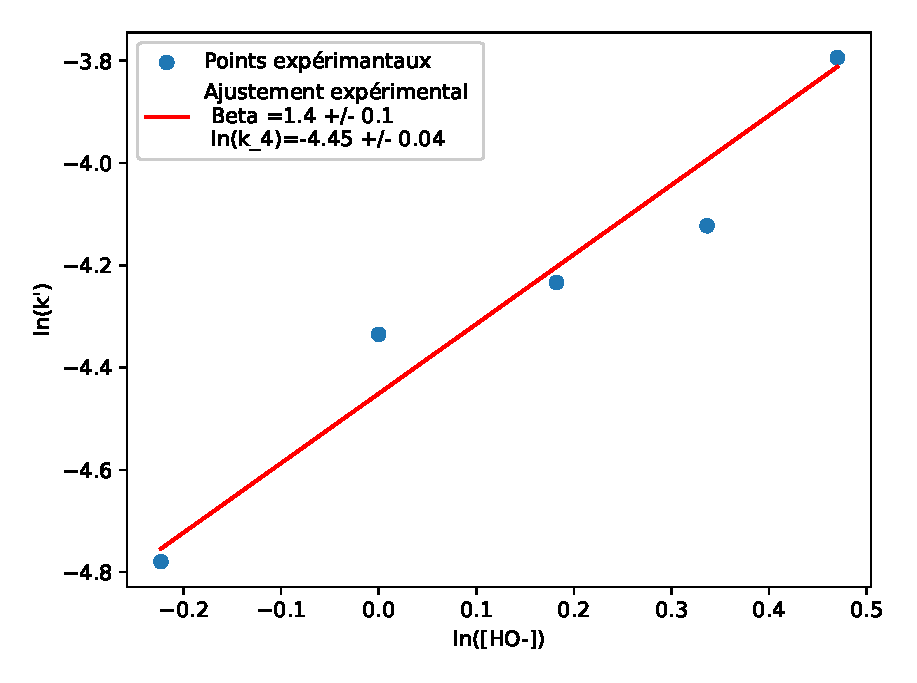
\includegraphics[scale=0.8]{Ln(k)2.eps}
        \caption{Graphique de ln(k') en fonction de ln([OH-]) à $4^\circ C$} 
        \label{im5:ln4 4 degré}
    \end{center}
\end{figure}

On obtient une valeur $k_{T2}=0.0117 \pm 0.0005 \ L.mol^{-1}.min^{-1}$.

\textbf{Question 5 et 6 :} On obtient une valeur $\beta = 1.4 \pm 0.1$, ce qui est cohérent avec la valeur trouvé pour la première expérience.

\textbf{Question 7 : } On calcule pour $[OH-]=1.4 \ mol.L^{-1}$ $t_{1/2}=\frac{ln(2)}{k'_{T2}}=\frac{ln(2)}{0.0162}=43 \ min$.

\textbf{Question 8 :} On a la relation :
\begin{align*}
    E_a &= -R \times ln \left(\frac{k_{T2}}{k_{T1}}\right) \left(\frac{1}{\frac{1}{T2}-\frac{1}{T1}}\right) \\
    E_a &= - 8.314 \times ln \left( \frac{0.0117}{0.055}\right) \left(\frac{1}{\frac{1}{277} - \frac{1}{293}}\right) \\
    E_a &= 6.13 \ kJ.mol^{-1}
\end{align*}

\textbf{Question 9 :} Dans ce travail pratique nous avons déterminer les ordes partiels d'une réactions, en vérifiant qu'ils ne changaient pas en fonction de la température.
Nous avons aussi déterminer les constantes de vitesses de la réaction pour différentes température, ce qui nous a permis de calculer l'énergie d'activation de la réaction.
Pour améliorer nos expériences, il faut améliorer notre détermination du coefficient d'extinction molaire, en réduisant le temps entre le début de la réaction et notre première mesure d'absorbance.
On peut aussi améliorer nos résultats en améliorant le contrôle de la température et en calculant les données pour plus de température différentes.

\end{document}